\subsection{Super Capacitor}
As explained in the Load System's analysis, in section \vref{sec:LoadSystemAnalysis}, the Generator's internal armature has an inductive reactance. This causes the Generator to resist a sudden change in current which isn't desirable due to the switching application of the MOSFET.

The problem can be solved by placing a Super Capacitor in parallel with the Generator. As the MOSFET turns off the Generator will impede the change and continue to produce current. This current is then used to charge the capacitor. When the MOSFET turns back on, the Generator will once again impede the change and the state of the current production will be inert. The current can then instead be drawn from the charged capacitor.

% Skriv om ting

\textbf{Calculations - Capacitance}\\
The size of the Super capacitor can be found by the largest specified voltage-drop above it - i.e the largest voltage-drop generated by the Generator. According to the Generator's analysis, in section \vref{sec:GeneratorAnalysis}, this voltage is generated at AU2's cruise speed and is equal to:
\begin{equation}
	V_b = \SI{18.16}{\volt}
\end{equation}
 %%
 
The biggest allowed voltage-drop over one switching-period can be calculated as the difference between the two values above:
\begin{equation}
	dV = V_b - V_{b,minimum} = \SI{18.16}{\volt} - \SI{16.13}{\volt} = \SI{2.03}{\volt}
\end{equation}
 
The MOSFET's switchfrequency f\textsubscript{switch} is chosen to be equal to \SI{20}{\kilo \hertz}. The time between each switch can then be calculated as:
\begin{equation}
	dt = \frac{1}{f_{switch}} = \frac{1}{\SI{20}{\kilo \hertz}} = \SI{0.05}{\milli \second}
\end{equation}

The minimum value of the Super Capacitor's capacitance can be found using the capacitor-formula below and the values found above:
\begin{equation}
	\begin{split}
		I &= C \cdot \frac{dV}{dt}\\
		\\
		\SI{13.484}{\ampere} &= C \cdot \frac{\SI{2.03}{\volt}}{\SI{0.05}{\milli \second}} \quad \Rightarrow \quad C = \SI{333}{\micro \farad}
	\end{split}
\end{equation}

The chosen type of super capacitor is a Epcos B41570 Aluminum electrolytic capacitor. This capacitor has a capacitance of \SI{10}{\milli \farad} and is rated to be able to handle a DC-voltage of \SI{100}{\volt}. The chosen capacitor has a much larger value than the one needed. However, this will only cause the voltage-drop dV to be much smaller than the required. The new voltage-drop can be found as:
\begin{equation}
	\begin{split}
		I &= C \cdot \frac{dV}{dt}\\
		\\
	\SI{13.484}{\ampere} &= \SI{10}{\milli \farad} \cdot \frac{dV}{\SI{0.05}{\milli \second}} \quad \Rightarrow \quad dV = \SI{67}{\milli \volt}
	\end{split}
\end{equation}

\textbf{Calculations - Power}\\
Due to the non-ideal nature of the capacitor it will contain both a resistance and a reactance. This means that both an active an a reactive power will be generated in the Super Capacitor. The active power can be calculated using the capacitor's equivalent series resistance (ESR):
\begin{equation}
	P_C = I_{C,rms}^2 \cdot ESR
\end{equation}

Where I\textsubscript{C,rms} is the rms-value of the current in the Super Capacitor. This value will be largest when MOSFET is operating with a duty-cycle of precisely 50\% and the Generator is generating the largest possible voltage. The power in the Load can then be found as:
\begin{equation}
	I_{load} = \frac{V_b}{R_{load}} \cdot 0.50 = \frac{\SI{18.16}{\volt}}{\SI{1.1065}{\ohm}} \cdot 0.50 = \SI{8.255}{\ampere}
\end{equation}

This current will be drawn from the capacitor when the MOSFET is on and the flow back into it when the MOSFET is off. If it is assumed that this change in direction happens instantaneous, then the current in the capacitor over a period T can be described using the following function:
\begin{equation}
	I_c(t) = I_{load} - 2 \cdot I_{load} \cdot u \left( t - \frac{T}{2} \right)
\end{equation}

Where u(t) is the unit-step-function. For a square-waved signal the rms-value can be found as the amplitude of the signal which is \SI{8.255}{\ampere}. Furthermore, the chosen capacitor is rated to have an equivalent series resistance (ESR) of \SI{15}{\milli \ohm}. The active power generated in the capacitor can therefore be calculated as:
\begin{equation}
	P_C = I_{C,rms}^2 \cdot ESR = (\SI{8.255}{\ampere})^2 \cdot \SI{15}{\milli \ohm} = \SI{1.022}{\watt}
\end{equation}

\textbf{Calculations - RLC-filter}\\
The coupling between the Generator and the Super Capacitor creates a low-pass RLC-filter due to the internal impedance in the Generator. The filter is seen below:

\begin{figure}[H]
	\centering
	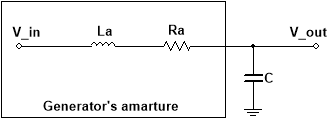
\includegraphics[width=0.5\linewidth]{Hardware/LoadSystem/RLC_filter}
	\caption{RLC-filter consisting of the Generator and the Super Capacitor}
	\label{fig:RLC_filter}
\end{figure}

The filter's transfer function in the s-domain can be found using the Laplace-transform. Using circuit-analysis the function below is found: 
\begin{equation}
	G(s) = \frac{1}{CLs^2 + CRs + 1}
\end{equation}

 The filter's frequency-response (bode plot) as well as the cutoff-frequency can be calculated using the specified values for the capacitance, resistance and the inductance.
\begin{equation}
	\begin{split}
		L_a &= \SI{0.072}{\milli \henry}\\
		R_a &= \SI{103}{\milli \ohm}\\
		C &= \SI{10}{\milli \farad}\\
		\\
		f_c &= \frac{1}{\sqrt{L_a \cdot C}} = \frac{1}{\sqrt{\SI{0.072}{\milli \henry} \cdot \SI{10}{\milli \farad}}} = \SI[per-mode=fraction]{1178}{\radian \per \second} = \SI{187.6}{\hertz}
	\end{split}
\end{equation}

\begin{figure}[H]
	\centering
	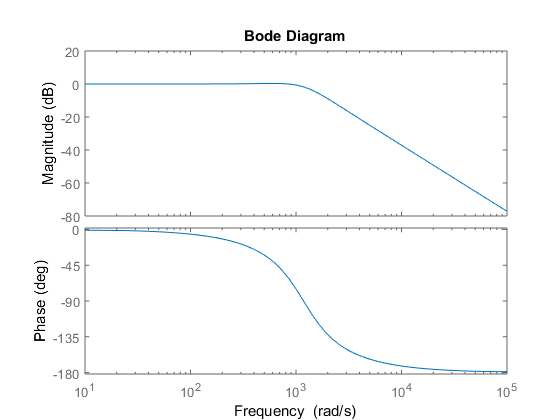
\includegraphics[width=0.7\linewidth]{Hardware/LoadSystem/BodeFilter}
	\caption{RLC-filter consisting of the Generator and the Super Capacitor}
	\label{fig:RLC_filter}
\end{figure}

Using the filter's transfer function it can be found that the amplification at the switching frequency f\textsubscript{switch} of \SI{20}{\kilo \hertz} is equal to \SI{-80}{dB}. At such high damping the output-current can effectively be assumed to be a steady DC-value.